\documentclass[12pt]{article}
\usepackage{graphicx} %for pictures
\usepackage{listings} %for code blocks
\usepackage{hyperref} %for hyperlink in ref and cite
\usepackage{fullpage}
\usepackage{parskip}

\graphicspath{ {../pics/} }

\title{Layer 2 blockchains for videogames}
\author{Lapo Falcone \\ lapofalcone@gmail.com}

\begin{document}
\maketitle
\tableofcontents

\newpage

\part{Blockchain concepts and their limitations} \label{part:bcatl}
In the last 3 decades internet has become a service used by virtually everyone. The framework which allowed the spread of the internet has been the \textit{client-server} paradigm.
Its success must be attributed to some important properties it guarantees, first and foremost the relative ease of implementation and maintainability of such solutions compared to others, such as peer-to-peer architectures.
Moreover, client-server solutions can achieve high performance and efficiency, by handling a lot of requests thanks to the power of ad-hoc hardware and replication. 
Another key characteristic of client-server is the fact that the owner of the service can fully control it, and change it based on his needs, as long as he follows the laws of the region he operates in and possible commitments he made with the users.

Despite all the positive properties of the client-server paradigm, there are some situations for which it is not suitable. 
What if we cannot trust the service provider? What if we want a service that is fully transparent for the users? What if we want a strong guarantee that data won't be modified?

In all these cases, and more, blockchain technologies are more suitable.

\emph{In the next sections we will briefly describe how a blockchain works, why it can be useful in videogames, and what are the main limitations which have prevented its use in the video gaming industry so far.}

\section {What is a blockchain} \label{section:wiab}
A blockchain, as the name suggests, is a chain of blocks. Each block contains transactions, which, in the simplest form, are exchanges of tokens between 2 users.

What actually creates the bond between 2 contiguous blocks of the chain, is the fact that each block also contains the hash of the previous one in the chain.

Blockchains are decentralized and distributed because the record of all the existing blocks (and therefore their relative \textit{position} in the chain) are not stored in a single, central server owned by some company. 
Indeed they are stored by the participants of the blockchain itself.

Since all the existing blocks are stored somewhere\footnote{Not every node stores the full history of blocks, only full nodes do \cite{bitcoin_full_nodes}.}, it is possible to reconstruct the tokens owned by each user.

In order for such a distributed ledger to work in a useful way, there is the need for a method to ensure 3 basic properties:
\begin{itemize}
    \item The transactions in a block must be valid.
    \item There must be an agreement among all the participants to the blockchain about the content (and therefore the order) of the blocks in the chain.
    \item Once a block has been added to the chain, it cannot be modified.
\end{itemize}

\subsection{Transactions} \label{subsection:transactions}
Each user of the blockchain is identified only by a pair of private and public keys \(<p_k, P_k>\).

A transaction is a \textit{packet} of data like this\footnote{In Bitcoins things are more complex than this. A user can spend an old transaction if he has a script to \textit{redeem} it. To spend a transaction he must provide the script to \textit{redeem} it and a script to re-lock it. Moreover, a user can merge many old transactions into a single one and can split the output by locking portions of it with different scripts. \cite{bitcoin_transactions}}:
\begin{table}[h]
    \centering
    \begin{tabular}{|c|c|c|c|}
        \hline
        Sender \(P_k\) & Receiver \(P_k\) & Amount & Sender signature \\
        \hline
    \end{tabular}
    \label{table:transaction}
\end{table}

For example, if the user with public key \verb|0x1234| and private key \verb|0x5678| wants to send 3 tokens to the user with public key \verb|0xabcd|, the transaction will look like this:
\begin{table}[h]
    \centering
    \begin{tabular}{|c|c|c|c|}
        \hline
        0x1234 & 0xabcd & 3 & sign(0x1234, 0xabcd, 3, 0x5678) \\
        \hline
    \end{tabular}
    \label{table:transactionExample}
\end{table}

Where \verb|sign| is a function to sign the transaction with the private key of the sender.

The signature is crucial since it guarantees authentication, integrity and non-repudiation of the transaction.

Once a user creates a transaction, it sends it to the miners network.

\subsection{Miners} \label{subsection:miners}
The role of the miners is to guarantee the validity of the transactions, create blocks and agree on the content of each block in the chain.

When a miner receives a transaction, he propagates it to the other miners. Each miner keeps the transaction it receives in a pool, then he chooses\footnote{Fees \cite{bitcoin_fees} play a key role in the way transactions get chosen.} a number of transactions to include in the next block.

All the transactions in a block must be valid, therefore the miner must check that:
\begin{itemize}
    \item The signature of the transaction is valid.
    \item The transaction is not already present in a previous block of the blockchain.
    \item The sender actually owns enough tokens to complete the transaction.
\end{itemize}

When a block of transactions is created, the miner adds the hash of the previous block of the chain to it.

Now the miner must solve a computationally complex puzzle and then send the block to the other miners.

If the solution to the puzzle is correct, and all the transactions in the block are valid, all the other miners will accept the block as the last block of the chain.

\subsection{Proof of work} \label{subsection:pow}
If miners could add any block they create to the blockchain, it would be impossible to obtain a consensus between the miners on what blocks are actually part of the chain.

For example, it would be impossible to have a consistent state of the blockchain among all the participants, due to the CAP theorem \cite{CAP_theorem}.

The blockchain wouldn't even be immutable, since it would be easy to replace an old block with another one.

For these and many other reasons, there must be a consensus mechanism among miners, in order to agree on what blocks are part of the chain.

The chronologically first consensus mechanism that has been used in a blockchain is proof of work (PoW) \cite{bitcoin_seminal}: after a miner creates a block of transactions, it has to add a \textit{number} to it, such that the hash of the whole block starts with a predefined amount of zeroes.
Since the hash is a non-invertible function, the only way to find a number with the property described above is brute force.

This simple mechanism solves the problems we discussed before. Indeed, now, it requires a lot of resources to modify an old block of the chain: not only a malicious miner should re-compute the hash of the block he wants to change, but also the hashes of all the blocks after it (since each block contains the hash of the previous one, which has changed).

Moreover, PoW reduces the number of blocks that can be created in a given interval of time, making it possible to reach a consistent state among the majority of miners\footnote{It is still possible that 2 miners solve different blocks at roughly the same time. In this case, the blockchain will have a branch. After some time one of the 2 branches will be longer than the other, because it is unlikely that the 2 branches evolve at the same speed. At this point, the longer branch will be the one chosen by the miners, and the other one will be discarded.}.

In order to make PoW work with faster hardware, it is possible to collectively choose the amount of required leading zeroes in the hash of the new proposed block.

Moreover, miners can add their address in a field of the block, so that they get rewarded for their work if they are able to create a new block.

\subsection{Journey of a transaction} \label{subsection:joat}
Here we make a summary of the steps that a transaction must follow to be included in the blockchain:
\begin{enumerate}
    \item User \verb|A| creates a transaction \verb|T|, signs it and sends it to the miners network.
    \item A miner \verb|M| receives \verb|T| and forwards it to the other neighboring miners.
    \item \verb|M| receives many other transactions, then creates a block \verb|B| with only valid transactions, among which \verb|T|.
    \item \verb|M| adds the hash of the last block of the chain and his address for the reward to \verb|B|.
    \item \verb|M| starts trying different numbers until it finds a number that satisfies the PoW requirements.
    \item \verb|M| forwards the new block \verb|B| to the other miners. 
    \item The other miners check the validity of \verb|B|, if it is valid they will consider it the last block of the chain, else they will simply ignore it.
\end{enumerate}

\subsection{Blockchain programmability} \label{subsection:programmability}
Until now we have seen a blockchain where simple users can exchange some currency with plain transactions. Bitcoin is an example of a blockchain with these characteristics.

More recently a new kind of programmable blockchains has arisen, whose main exponent is Ethereum. 

The core concepts of a programmable blockchain like Ethereum are similar to the ones of a \textit{plain} one, with 2 main additions\footnote{Another evident difference of Ethereum is that it now uses proof of stake, but it is not important in this context.}:
\begin{description}
    \item[Smart contracts] Blockchain wallets controlled by an immutable script.
    \item[Account-based model] Nodes keep the blockchain state in a \textit{table} like the one in \ref{table:account_based_state}. A transaction can now be defined as an argument in a state transition function: 
    \[\mathcal{N} (state_{old}, transaction) = state_{new}\]
\end{description}

\begin{table}[h]
    \centering
    \begin{tabular}{|c|c|c|l|l|}
        \hline
        \textbf{Address} & \textbf{Balance} & \textbf{Nonce} & \textbf{Code} & \textbf{Storage} \\
        \hline
        0x1234 & 3 & 149 & & \\        
        0xabcd & 101 & 74 & \verb|if(bal > 0) then sendMoney(...)| & bal = 23 \\
        \hline       
    \end{tabular}
    \caption{Simplified example of the account-based state}
    \label{table:account_based_state}
\end{table}

A smart contract is deployed via a transaction, where its source code is specified.

Other users of the blockchain can interact with a smart contract by sending transactions where they specify the interface function to call and the necessary arguments.

When such a transaction is included in a block, the validator must also execute the code specified by the smart contract, whose execution, being deterministic, can be checked by the other validators. All validators should reach the same state.

Each smart contract has associated storage, which is part of the state of the blockchain and can be read and written during execution.

Smart contracts are immutable, which means it is not possible to change, or even delete, the code of the smart contract after it is deployed. 
This property is particularly relevant because it means that a user can be sure of what will happen if he interacts with a smart contract, by simply reading the smart contract code.

Another important aspect of smart contracts are execution fees. A smart contract will be executed by a validator, and the more complex the smart contract is, the more resources and time the validator will have to use.

For this reason, when a transaction is created, it is necessary to specify a maximum fee that the validator will earn by including the transaction in the block.
Each instruction in a smart contract has an associated fee. If during the execution the total fee exceeds the maximum fee specified in the transaction, the execution will be aborted.

There are 3 main types of resources that require fees during the execution of a smart contract:
\begin{description}
    \item[Computation] The instructions executed.
    \item[Calldata] The arguments passed in the transaction.
    \item[Storage] The cost of writing to the smart contract storage.  
\end{description}

\subsection{Tokens} \label{subsection:tokens}
Smart contracts can be used to implement tokens, which are virtual assets that can be owned by the accounts.

Tokens differ from the currency of the blockchain (e.g. Bitcoin or Ether) because they are generally used in a closed environment and serve a specific purpose (for example a certain token could signify membership to a certain organization).

There exist 2 kinds of tokens:
\begin{description}
    \item[Fungible tokens] A token is indistinguishable from another one, and it can be fractioned. 
    \item[Non-fungible tokens] A token has a unique identifier and value, it cannot be fractioned. 
\end{description}

\section{Why blockchain can be used in videogames} \label{section:wbcbuiv}
In the previous sections, we have briefly seen how a blockchain work. Now we will see why it can be used for videogames.
\begin{description}
    \item[Ownership of digital assets] A videogame could reward the player with NFTs. This would be different than rewarding a player with a game-specific item, because the player would own the NFT independently from the game, and would even be free to sell it for fiat money.
    \item[Cross compatibility] If players are rewarded with tokens, it would be easier for other games to integrate them. In this way, players could easily import and use items earned in one game in another one.
    \item[Transparency] One of the key characteristics of blockchains is transparency. All transactions are public, therefore it can potentially be easier to detect cheaters in a competitive environment. Blockchain would also make it impossible for software houses to censor some players.
    \item[Fairness] Smart contracts could be used to create a fair ground between the software house and the player base, for example by using smart contracts to implement loot boxes.  
\end{description}

\section{Why blockchain cannot be used in videogames} \label{section:wbcnbuiv}
Blockchain can be used in videogames at different stages.

Most blockchain-powered videogames today are using blockchain as a storage for in-game rewards. This means that the execution of the game happens off-chain (generally on a server), but the server can decide to reward a player with on-chain tokens.

This paradigm is useful to implement the ownership of digital assets, and, to some extent, cross-compatibility, but it doesn't help with transparency and fairness.

To achieve transparency and fairness the game itself should be executed inside a smart contract on the blockchain.

There are 2 main issues with doing so:
\begin{description}
    \item[Costs] Usually the main loop of a videogame is quite complex. This means that the fees for executing the smart contract will be high.
    \item[Scalability and performance] Blockchains have a much lower throughput than client-server solutions. This is an inherent characteristic of blockchain as we know it nowadays, and, as we have seen, a core principle of their functioning.
\end{description}

In recent years a new framework that can help with both issues has emerged: blockchain layer 2 \cite{ethereum_scaling}.

\newpage

\part{Blockchain layer 2} \label{part:bl2}
As we have seen in \ref{section:wbcnbuiv} layer 1 blockchains suffer from high fees and poor scalability.

This is a direct consequence of the blockchain trilemma \cite{blockchain_trilemma}, which states that we can have only 2 out of distribution, security and scalability.
To try to tackle these issues layer 2 blockchains have been invented.

The core idea behind layer 2 is to transfer as much load as possible outside of the blockchain, and use the layer 1 properties only to finalize the operations that happened off-chain.

They try to do so by starting from a predefined state, usually stored in a smart contract, bundling up many transactions off-chain, and eventually reporting to the smart contract what happened off-chain \cite{ethereum_layer2}.
The smart contract can verify that some predetermined rules have been followed during the off-chain operation. 

The off-chain transactions can be faster because they don't have to involve all the nodes of the blockchain to be verified, and can resort to simpler verification protocols that scale better and are more suited for certain applications.

\emph{In the next sections we will explore some of the most used layer 2 approaches, and we will find out why ZK rollups are arguably the best solution for videogames.}

\section{Off-chain state channels} \label{section:ocsc}
The core idea behind state channels is to let channel participants perform transactions off-chain, and only submit 2 on-chain transactions to open and close the channel.

The lifecycle of a channel is made up of 3 phases \cite{ethereum_state_channels}:
\begin{description}
    \item[Opening] To open a channel all the participants must add funds to a smart contract and agree to the initial state by signing it.
    \item[Usage] Once a state channel is open, participants can start exchanging transactions off-chain. A transaction looks like this:
        \begin{table}[h]
            \centering
            \begin{tabular}{|c|c|c|c|}
                \hline
                Old state & New state & Transaction to go from old state to new state & Nonce \\
                \hline
            \end{tabular}
            \label{table:state_channel_transaction}
        \end{table}

        A transaction to be considered final must be valid (i.e. following the rules stated in the smart contract, such as not spending more than what you own) and signed by all parties in the channel.
        If a transaction is valid, it cannot be reverted.
    \item[Closing] Any participant can decide to send a transaction to the smart contract on layer 1. At this point, a challenge period starts, where the other parties can send a transaction to challenge the one proposed by the first participant.
    
                    For example, if user \verb|A| wants to finalize the state channel with an old transaction, and user \verb|B| has a newer transaction signed by all the parties, he can use the newer transaction to prove that user \verb|A| is malicious.
                    In this case user \verb|A| would lose all the funds he added to the smart contract of the state channel.

                    The presence of the challenge period enhances the security of honest users: they can challenge malicious parties and they can withdraw their funds if other parties stop responding.

                    In any case, at the end of the challenge period, funds in the state channel are distributed based on the last valid transaction sent to the smart contract.
\end{description}

It is important to note that the state of a channel doesn't only hold currencies, but also any other possible variable. For this reason, state channels can be used to run computation off-chain.

\subsection{State channels and videogames} \label{subsection:scav}
As we have seen state channels rely on layer 1 blockchain to guarantee liveness (the smart contract for the channel is always available), security and finality (as soon as a transaction is signed by everyone, it is not revertible).

Moreover, since they allow off-chain computation, state channels don't suffer from the scalability and performance issues typical of blockchains.

On the other hand, in a video gaming context, state channels do not guarantee the transparency and fairness properties we are looking for.

For example, let's imagine we have a state channel to play a game of chess against a computer, where you get a reward if you win. The state channel would be initialized and signed by the player and the server where the chess engine runs.
Then the player and the server could start exchanging transactions to move pieces. Let's now say that the player is one move away from checkmate, and the server refuses to acknowledge the transaction that delivered checkmate.
The player cannot send the checkmating transaction to the layer 1 smart contract, because the server could challenge it with the last co-signed transaction. And in this framework it would be impossible to prove that the server did it intentionally, maybe it simply didn't receive the transaction.

Therefore this solution wouldn't be much different than a simpler client-server solution with on-chain storage.

\section{Sidechains} \label{section:sidechains}
Sidechains are independent blockchains that can interoperate with the layer 1 blockchain.

Being separate, sidechains can use different consensus mechanisms than the main blockchain. On the one hand, this can help with performance, scalability and fees cost, but, on the other hand, the sidechain may lose some important guarantees of the layer 1 blockchain.
For example, a sidechain could trade distribution for scalability to satisfy the blockchain trilemma and be scalable.

Sidechains can communicate with the blockchain via bridges.

Bridges are mechanisms that allow to connect different blockchains, allowing users to transfer assets between them \cite{ethereum_bridges}.

There are many types of bridges, one of the most used kind locks or burns items in one blockchain and mints the same item in the other one, in order to simulate the transfer.

\section{Rollups} \label{section:rollups}
Rollups are mechanisms where multiple transactions are performed off-chain and aggregated in a single batch transaction which is submitted to a smart contract on the layer 1 blockchain.

Off-chain transactions are executed in a layer 2 blockchain, where the validators (also called sequencers) also have the task to send batches of layer 2 transactions to the layer 1 smart contract.

Based on the mechanism that is used to determine the validity of the transactions in the batch, it is possible to categorize rollups into optimistic and zero-knowledge.

\subsection{Optimistic rollups} \label{subsection:optimistic_rollups}
The main assumption of optimistic rollups is that the majority of the transactions inside a batch are valid, therefore sequencers can send the new state of the layer 2 blockchain to the layer 1 smart contract, without any validity proof.

The caveat is that the layer 1 smart contract will wait a challenge period (usually 7 days) before accepting the new state. 
During this period other participants to the layer 2 blockchain can send fraud proofs to challenge the new state sent by the sequencer.

This mechanism enables better scalability and cost efficiency than in layer 1 blockchains, since smart contracts can be executed on layer 2, and the layer 1 fees are split among all the transactions in a batch.

\subsubsection{Entering an optimistic rollup} \label{subsubsection:entering_optimistic_rollup}
To enter a rollup a user must deposit some assets (generally tokens) in the layer 1 rollup smart contract. These assets are then transferred to the layer 2 blockchain via a bridge to a specified address.

At this point, the user must wait until the transaction made by the bridge to the specified address gets processed by the sequencer and sent in a batch to the layer 1 smart contract.

\subsubsection{Exiting an optimistic rollup} \label{subsubsection:exiting_optimistic_rollup}
To exit a rollup a user must send an exit transaction to the layer 2 sequencer. The sequencer will execute the transaction by burning all the assets of the user (that should be included in the exit transaction), and then include this transaction in a batch.

At this point, the user must to generate a cryptographic proof (generally a Merkle proof) to show that the exit transaction was inside the last batch, and that the layer 2 account that submitted such transaction belongs to the user.

Now it is possible to send the proof to the layer 1 smart contract, along with an address where to send the withdrawn assets.

\subsubsection{L2 - L1 interaction} \label{subsubsection:l2l1i}
The sequencers store the state of the rollup as a Merkle tree (see section \ref{section:merkle_trees}). The root of such tree is also stored in the layer 1 smart contract. \cite{optimistic_rollups}.

When a sequencer wants to send a batch to the layer 1 smart contract, it must send a transaction containing:
\begin{itemize}
    \item The Merkle root of the old state.
    \item The Merkle root of the new state.
    \item An highly compressed summary of all the transactions in the batch (containing also the input data of the transactions).
    \item The Merkle root of the transactions in the batch.
\end{itemize}

The layer 1 smart contract receives the transaction and compares the Merkle root of the old state with the one in its storage. If they match, the Merkle root in the storage is updated to the Merkle root of the new state.

The highly compressed list of all the transactions and their inputs won't be part of the layer 1 state, but it will simply be stored as calldata, for cost reasons.

The Merkle root of the transactions in the batch is necessary in order to let other participants prove that their transaction is part of the batch (for example when a user wants to withdraw assets from the rollup).

At this point, the challenging period begins, and other users can send fraud proofs. 2 main proving schemes can be adopted:
\begin{description}
    \item[Single round] In this scheme all the transactions' inputs being part of a batch must be stored (as calldata) in the layer 1 smart contract. Since the smart contract has all the transactions and their inputs, it can replay them and verify whether the new state Merkle root matches with the one sent by the sequencer.
    \item[Multi round] This proving mechanism is more complex but also more efficient. In this case, only the Merkle root of the summary of transactions is required be stored as calldata.
                        
                        The process to prove fraud consists of a dialogue between the sequencer and the challenger, supervised by a layer 1 smart contract. At each step the asserter must split computation performed in a batch into 2 equal halves and state the output\footnote{With output here it is intended the hash of the full state of the computation till this point} of each one of the 2 halves. The challenger can decide which half he wants to challenge.
                        This process goes on until only a single instruction remains in the asserter computation. At this point, both the asserter and the challenger must send their prediction for the outcome of that instruction, which is executed by the layer 1 smart contract, which can easily find out who is lying. This process can be visualized in Figure \ref{figure:multi_round_fraud_proof}.

                        Since we have the Merkle root of the batch and all the transactions in the layer 2 blockchain are available to other users, the challenger can prove whether a specific part of the computation shouldn't be there by hashing all the transactions that were actually included in the block. 
                        And in case the sequencer and the challenger agree on the computation, the proof we described above is enough to understand who is lying about the new state.
\end{description}

\begin{figure}[h]
    \centering
    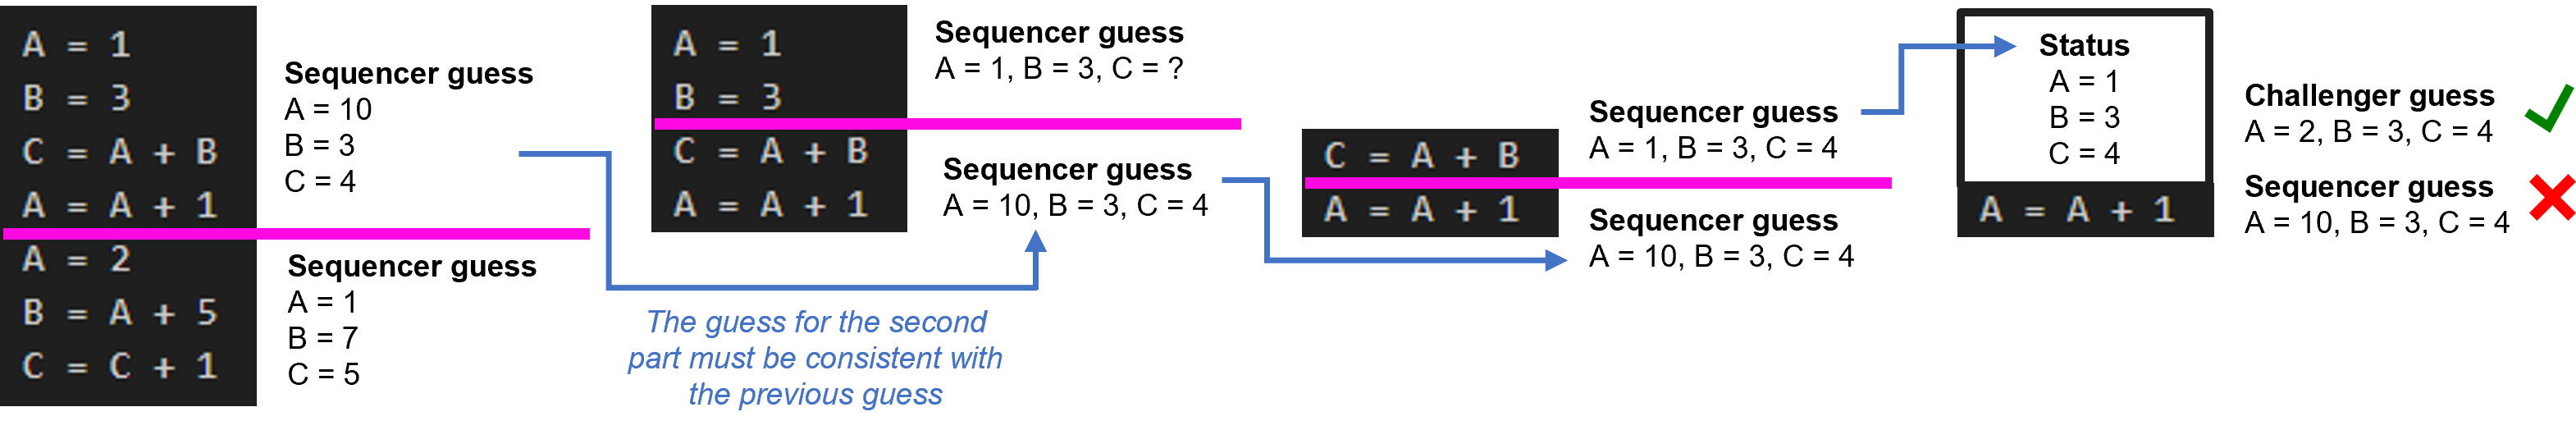
\includegraphics[width=\textwidth]{multi_round_fraud_proof}
    \caption{The multi round fraud proof mechanism visualized}
    \label{figure:multi_round_fraud_proof}
\end{figure}

\subsubsection{Optimistic rollups and videogames} \label{subsubsection:orav}
Optimistic rollups are a step in the right direction towards the use of the blockchain in videogames.

Indeed they do not suffer from the transparency and fairness problems we discussed in section \ref{subsection:scav}, and, at the same time, they maintain more security and decentralization guarantees than sidechains, since they maintain a strict bound with the layer 1 blockchain.

The main problem of the majority of the implementations of optimistic rollups are:
\begin{description}
    \item[High fees] Even if fees are lower than using a layer 1 blockchains, the need to send all the transactions and their inputs in a batch (although compressed) as calldata, isn't enough to lower the fees enough for adoption in the video gaming world.
    \item[Withdrawal time] As we have seen in section \ref{subsubsection:exiting_optimistic_rollup}, it takes a very long time (usually 7 days) to be able to withdraw the assets from an optimistic rollup. This doesn't pair well with the cross compatibility property, since different games will most likely run on different optimistic rollups implementations.
\end{description}

\subsection{Zero-knowledge rollups} \label{subsection:zk_rollups}
Zero-knowledge rollups are a layer 2 scaling solution that operates similarly to optimistic rollups. Therefore, as in optimistic rollups, the layer 2 sequencers receive various transactions, execute them and only update the layer 1 smart contract when a batch of transaction has been executed.

As in optimistic rollups, this mechanism improves scalability and performance of the blockchain, and splits the layer 1 fees among all the transactions in a batch.

The core difference between optimistic rollups and ZK rollups is in the way the transaction batch update gets validated in the main blockchain.

Sequencers of ZK rollups must send a zero-knowledge proof along with the changes to the old state. The zero-knowledge proof is a cryptographic demonstration that the proposed changes to the state are actually the result of executing all the transactions in the batch.

This change makes it so that it isn't required to store a compressed summary of the transactions' inputs on the layer 1 chain as calldata, greatly lowering the fees needed. Moreover, the layer 1 smart contract can immediately verify whether the changes are valid, so the challenge period can be completely removed.

\subsubsection{Entering a ZK rollup} \label{subsubsection:entering_zk_rollup}
The process to enter a ZK rollup is very similar to the one described in \ref{subsubsection:entering_optimistic_rollup}.

The user must deposit some assets in the layer 1 smart contract, a bridge will transfer the assets to the rollup. After the sequencer adds the transfer transaction to a batch, the user will be able to use his assets in the ZK rollup.

\subsubsection{Exiting a ZK rollup} \label{subsubsection:exiting_zk_rollup}
If the process to enter a ZK rollup is basically the same as the one to enter an optimistic rollup, the exiting process shows some differences caused by the different way in which transaction batches are verified in layer 1.

To exit a ZK rollup a user must initiate an exit transaction by sending all his assets to a specific burn address.

As soon as this transaction is added to a batch by the sequencer, the user must create a Merkle proof to prove the presence of the exit transaction in the batch.

Then he can send a withdrawal request to the layer 1 smart contract with the following information:
\begin{itemize}
    \item The Merkle proof.
    \item The exit transaction data.
    \item The Merkle root of the transaction batch containing the exit transaction.
    \item A layer 1 address where to deposit the withdrawn assets.
\end{itemize}

The layer 1 smart contract can hash the transaction data and use the Merkle proof to verify that such transaction is indeed part of the Merkle root of the batch. If this is the case the smart contract will deposit as many assets as those burned in the exit transaction to the specified layer 1 address.

This process has a way lower latency than the one used for optimistic rollups, because the challenging period doesn't exist in ZK rollups.

\subsubsection{L2 - L1 interaction} \label{subsubsection:zk_l2l1i}
Similarly to optimistic rollups, the sequence must compute the Merkle tree of the state of the rollup, and send its root along with:
\begin{itemize}
    \item The Merkle root old state. 
    \item The transactions (this time without inputs).
    \item The validity proof. 
    \item The Merkle root of the transactions in the batch. 
\end{itemize} 

To the layer 1 smart contract.

When the smart contract receives the batch, it will execute the validity proof, check the old state and, if everything matches, update the rollup Merkle tree root in its storage.

\subsubsection{Intuition on the validity proofs} \label{subsubsection:iotvp}
Validity proofs are complex cryptographic objects which allow to demonstrate the truthfulness of a statement based on a computation in way less time than executing the full computation.

\paragraph{From computation to polynomial}
The first step towards these proofs is to create a process able to associate a computation with a polynomial.

To do so it is possible to convert the computation into an arithmetic circuit, which is a representation of the computation similar to a control flow graph. A circuit is made up of inputs, intermediate nodes, a root node and edges connecting the nodes.

It is now possible to specify the inputs, and save the results after the operation specified in each node in a table, called trace.

This trace will therefore contain numbers, which can be interpreted as points in a multidimensional space.

It is therefore possible to build a polynomial with the lower degree possible that passes through all the points in the trace.

\paragraph{}


\part{Appendix} \label{part:appendix}
\section{Merkle trees} \label{section:merkle_trees}
\cite{ethereum_merkle_trees} \cite{ethereum_merkle_proof}

\newpage
\bibliographystyle{apalike}
\bibliography{biblio}
\end{document}
